\documentclass[11pt]{article}
\usepackage{setspace}
\usepackage[a4paper]{geometry}
\usepackage{url}
\usepackage{graphicx}
\usepackage{paralist}
\usepackage{amsmath}
\usepackage{amssymb}
%\usepackage{mathtools}
\usepackage{amsthm}
\usepackage{mdwlist}
%\doublespacing



\newcommand{\HRule}{\rule{\linewidth}{0.5mm}}

\newtheorem{definition}{Definition}
\newtheorem{corollary}{Corollary}
\theoremstyle{definition}

%\newcommand{\qed}{\nobreak \ifvmode \relax \else
 %     \ifdim\lastskip<1.5em \hskip-\lastskip
 %     \hskip1.5em plus0em minus0.5em \fi \nobreak
 %     \vrule height0.75em width0.5em depth0.25em\fi}


\begin{document}


  \begin{titlepage}

    \begin{center}

      % Upper part of the page
       %\includegraphics[width=0.15\textwidth]{~/Dissertation/Reports/Deliverable1/logo.eps}\\[1cm]    

      \textsc{\LARGE Heriot-Watt University}\\[1.5cm]

      \textsc{\Large Final Year Dissertation -- Deliverable One }\\[0.5cm]


      % Title
      \HRule \\[0.4cm]
      { \huge \bfseries Fast Algorithms for Hard Problems}\\[0.4cm]

      \HRule \\[1.5cm]

      % Author and supervisor
      \begin{minipage}{0.4\textwidth}
        \begin{flushleft} \large
          \emph{Author:}\\
          Joseph Ray \textsc{Davidson}
        \end{flushleft}
      \end{minipage}
      \begin{minipage}{0.4\textwidth}
        \begin{flushright} \large
          \emph{Supervisor:} \\
           ~Dr. David \textsc{Corne} 
        \end{flushright}
      \end{minipage}

      \vfill

      % Bottom of the page
      {\large \today}

    \end{center}

  \end{titlepage}

  \begin{abstract}
    This document contained herein, constitutes the submission for deliverable
    one of the dissertation ``Fast Algorithms for Hard Problems" written by
    Joseph Davidson. It will introduce the notion of hard problems, outline
    the objectives of the investigation, strategies and testing methods. It
    also contains a literature review that aims to present the current state
    of research in the area. It will close with a projected timetable for the year.

  \end{abstract}
  \newpage

  \tableofcontents

  \newpage

  \section{Introduction}
    In Computer Science `hard' problems can be considered as those which are not contained within the
    intersection of the complexity classes P and NP (if $\text{P} \neq \text{NP}$).   Traditional computers (those consistent with the
    deterministic model of computation) can, in general, quickly find an exact solution to problems contained
    in the class P, but cannot do so for those which are outside P. This provides
    a problem for computer scientists, as the NP problems (defined in equation \ref{eq:NPproblems})
    are very interesting and useful problems that are considered intractable because of the
    time it would take to solve them \cite{Sipser:2005}. The best we can do for now is approximate an answer for these
    problems.

    This project is not looking to find a fast way to get exact answers for the NP problems
    but to investigate the usage of greedy
    algorithms and machine learning to quickly approximate solutions which can be considered `good enough'
    for the problem at hand.

    To do this, I will be investigating one specific problem: the \emph{vertex cover problem}\footnote{For a definition
    of the problem, see definition \ref{defVC} in section \ref{sec:VertexC}}. This problem has a useful property that 
    allows any fast approximation result to be used for any of the NP problems (see NP-completeness in section \ref{NPC}). 
    This property will, if the results of the investigation are favourable, allow me to generalise my approximation algorithm
    to the entirety of the class NP. 

    \subsection{Definition of NP}
      First, we will define the complexity class P. For this, will introduce the complexity class DTIME.
      \begin{definition}[DTIME]
        $\mathrm{\textbf{DTIME(f(n))}}$ is the class of decision problems\footnote{This is not strictly true. In complexity theory, Turing machines decide \emph{languages} instead of problems and the complexity classes are classes of languages decidable by certain Turing machines. I consider this a necessary abstraction however, as we are discussing algorithms for deciding these languages so we can refer to them as `problems'. This will be the convention for the rest of the dissertation.} solvable by a Turing machine in time $O(f(n))$.  
      \end{definition}
      We can now construct a definition of the class P by using DTIME\ldots
      \begin{definition}[P]
        $\mathrm{\textbf{P}}$ is the class of decision problems that are solvable by a deterministic Turing machine in polynomial
        time.
        \begin{equation}
          \mathrm{P} = \bigcup_{k}\mathrm{DTIME}(n^{k})
        \end{equation}
      \end{definition} 

      If $\text{P} \neq \text{NP}$ then we can view the `hard' NP problems as those that are not
      contained within the intersection of
      P and NP. However -- because of the unclosed nature of P vs NP -- we shall define the class NP in more concrete
      terms.
 
      \begin{definition}[NTIME]
        $\mathrm{\textbf{NTIME(f(n))}}$ is analogous to $\mathrm{DTIME(f(n))}$ as it is the class of decision problems solvable by
        a nondeterministic Turing machine in time $O(f(n))$. 
      \end{definition}   
      This definition allows us to state: 
 
      \begin{corollary}
        \begin{equation} \label{eq:NPproblems}
           \mathrm{NP} = \bigcup_{k}\mathrm{NTIME}(n^{k})
        \end{equation}
      \end{corollary}
    
    \subsection{Why NP problems are intractable}
      The term NP stands for ``Non-Deterministic Polynomial Time" which means
      that a non-deterministic computer is capable of solving a problem
      $n \in \text{NP}$  with an asymptotic upper bound time of: $ T(n) \in O(n^{x}) $ where $0<x$ and $x$ has a reasonable
      upper bound. 
      This time is referred to as ``Polynomial time" and we shall consider problems that
      can be solved in this time as tractable and problems that take longer as
      intractable.

      Up until very recently, non-deterministic computers were more of a convenient 
      mathematical model to help describe complexity classes. Quantum computers
      run with non-deterministic principles, but are in the very early stages of research \cite{website:quantum}.
      Consider a computation tree for NP decision problems, which is a tree that has branches for
      every decision point starting from the starting state at the root, ending with 
      either an accept or reject state at the leaves.

      We can picture a deterministic computer $D$ simulating a nondeterministic computer $N$ as performing
      a breadth first search, expanding each level of the tree until it finds an accepting state.
      On an input of length $n$, each branch of the computation tree has a length of at most $t(n)$. Each
      node in the tree can have at most $b$ children so we can deduce that the number of leaves in the tree is
      at most $b^{t(n)}$. We can use this to establish an upper bound on the total number of nodes in the tree:
      $O(b^{t(n)})$ because the total number of nodes in a tree cannot be more than twice the number of leaves.
      As said before, the time taken to expand a branch of the tree is at most $O(t(n))$ therefore, the running time for
      the deterministic computer $D$ is $O(t(n)b^{t(n)}) = 2^{O(t(n))}$ which we can generalise
      to $T(n) \in O(2^{n})$ \cite{Sipser:2005}.

      We can think of a non-deterministic machine using the same computation tree in two ways:

      \begin{itemize}
        \setlength{\itemsep}{1pt}
        \setlength{\parskip}{0pt}
        \setlength{\parsep}{0pt}
        \item A Machine that can expand entire tree levels in the same time it takes a deterministic machine to expand one node.
        \item A Machine that always expands tree nodes on an accepting path.            
      \end{itemize}
       
      In the first case, we can see that the non-deterministic machine is $t(n)$ times faster than the deterministic one.
      In the second, we can think of the non-deterministic machine as the luckiest deterministic machine in the
      universe because it always expands the correct nodes in the tree that lead to an accepting state \cite{Sipser:2005}.

      It is simple to see that for a problem space that is large (say $n=4000$), a deterministic machine would have a
      worst case running time of: $T(4000) \in O(2^{4000})$ which is unacceptable. Hence the need for fast algorithms
      for approximating the solution to many of these problems.  

      \subsection{NP--completeness} \label{NPC}
        There is a subset of the NP problems in which every problem in NP can be reduced to one of these problems. 
        This set is called the NP-complete problems, defined in equation \ref{eq:NPC} below.

        \begin{equation} \label{eq:NPC} 
          \text{NPC} = \{x\mid x \in \text{NP} \land (\forall y \in \text{NP}: y \prec x )\}  
        \end{equation}

        Where $x$ and $y$ range over the problems in NP and $y \prec x$ means: ``There exists a polynomial Karp reduction from $y$ to $x$" \cite{citeulike:Karp}\cite{citeulike:Cook}.

        The NP-complete problems are a good place to start finding a fast approximation algorithm because
        of the many-one reducibility property of the problems in the set. If a fast approximation algorithm can be found
        for one of the problems, that algorithm can be used as a subroutine for solving all of the other NP
        problems.

        The vertex cover problem itself is an NP problem, which is one of the motivations for it being the problem of
        choice for my investigation. If I were to find an algorithm that could solve the p

 
  \section{Project objectives}
    The main objective of this project is to attempt to determine a method of producing approximations for NP
    problems -- such as the vertex cover problem -- very quickly. Because the NP problems are a famous class
    in the field of complexity, many approaches have been
    tried to obtain optimal results quickly. These methods have a problem which is that they often
    depend on stochastic methods which generally do not produce results that are always reproducible,
    making multiple runs of the programs a necessity.
    My attempt at this problem will try to use more deterministic methods. The use of greedy algorithms for making
    fast approximations will be investigated.

    \subsection{Strategies}  \label{sec:Strat} 
      As mentioned above, there are many strategies that can be investigated with respect to finding a quick approximation
      for a vertex cover.
      The strategies that I wish to focus on in this investigation -- as well as reasons for choosing them -- are below.
      \begin{itemize}
        \setlength{\itemsep}{1pt}
        \setlength{\parskip}{0pt}
        \setlength{\parsep}{0pt}
        \item Greedy algorithms.
        \item Machine learning techniques -- such as Genetic algorithms or ANNs.
        \item Graph preprocessing.
        \item A combination of the above.
      \end{itemize}
      
      \subsubsection{Greedy algorithms} \label{sec:greedy}
        Greedy algorithms have been used extensively in the investigation into NP problems. 
        Due to their nature, some greedy algorithms are more successful than others -- for instance,
        I present below a very simple greedy algorithm to obtain an approximate vertex cover \cite{paper:hybrid}
          \begin{enumerate} 
            \setlength{\itemsep}{1pt}
            \setlength{\parskip}{0pt}
            \setlength{\parsep}{0pt}
            \item Given an undirected Graph $G = (V,E)$.
            \item Set $V' = \emptyset$.
            \item Repeat:
              \begin{itemize}
                \setlength{\itemsep}{1pt}
                \setlength{\parskip}{0pt}
                \setlength{\parsep}{0pt}
                \item Choose a vertex $v_{k}$ having the largest degree in $G$.
                \item Set $V'\triangleq V' \cup \{v_{k}\} $, $V \triangleq  V \setminus \{ v_{k} \} $, and $ E \triangleq E \setminus \{e\mid e \cap v_{k} \neq \emptyset \}$.
              \end{itemize}
             \item Until $G$ is empty.
          \end{enumerate}

        This algorithm simply selects the vertex with the highest degree in the graph, adds it to the vertex cover
        and then removes it from the graph, along with the edges incident with it. The algorithm  quickly produces
        a result in polynomial time, but the result is not very accurate.
        
        It is the eventual aim of this project to produce an algorithm that still quickly produces a result,
        but that result is also highly accurate. The usage of greedy algorithms is a possibility for achieving this goal,
        but it appears that there is a speed -- accuracy trade off for all such algorithms that attempt to
        solve NP problems. A balance will have to be struck to make greedy algorithms a viable solution. 

      \subsubsection{Machine learning} \label{sec:machine}
        Machine Learning techniques have been successfully applied to problems in many fields. Genetic algorithms have
        designed NASA antennae \cite{citeulike:NASA} and have been applied to solving the n-queens problem (another
        NP problem) \cite{queens}. Artificial Neural Networks have been used to autonomously control vehicles
        and studies have conducted into the effectiveness of these systems (see ALVINN \cite{BAL97a}).
  
        If an appropriate learning function can be devised, training these algorithms to produce
        optimal results could be a possibility. With the right implementation of these algorithms, all that
        would be needed is a reliable set of training examples. Xu, Boussemart et al. \cite{citeulike:XuSimple} have devised
        models that could be used to create hard NP instances with a fixed solution. These problems and answers
        can form the basis of training the learning algorithms using instance based learning (discussed in section \ref{PI}). 
      
      \subsubsection{Graph preprocessing} \label{sec:prePro}
        There are methods for preprocessing the input that may improve the chances of obtaining an optimal solution.
        A technique for this is \emph{Kernelization} \cite{paper:KernelIntro}. Kernelization works by removing clauses
        (in the case of the Satisfiability problem) that trivially have to be true in order for there to be an
        optimal solution.
        Possessing this knowledge allows us to shrink the input to a smaller equivalent by removing these clauses.
 
        Kernelization techniques were originally envisioned to be used more for programs that use brute force searching to
        find  solutions, but
        they may have applications to assist greedy algorithms that might get `confused' when searching for
        solutions in large search spaces.  
         

    \subsection{Problem selected} \label{sec:VertexC}
      As mentioned above, the problem that I have selected is the vertex cover problem which is defined below:
      \begin{definition}[Vertex Cover Problem] \label{defVC}
         Given an undirected graph $G = (V,E)$, find
        a subset $V' \subseteq V $ of minimum cardinality such that for each $e \in E$, $ e \cap V' \neq \emptyset$ holds \cite{paper:hybrid}. 
      \end{definition} 
      Informally: Given a Graph $G = (V,E)$, we aim to find a set $V'$ of the minimum number of
      vertices $v \in V$ required such that every edge $e \in E$ is adjacent to at least one vertex in $V'$.

      This problem has been demonstrated to be NP-complete by Karp \cite{citeulike:Karp} using a reduction from 
      the Satisfiability problem, first shown to be NP-complete by Cook \cite{citeulike:Cook}, to the problem of
      finding maximal cliques in a graph and then reducing the clique problem to the vertex cover problem.
      
      I have selected this problem primarily because I have previous experience with it and it
      is also one of the most studied problems in graph theory so there is a vast amount of background research
      to draw on.

            
  \section{Discussion of technical literature}
    The vertex cover problem is one of the most studied in graph theory. To this end, there is plenty of 
    technical literature on multiple aspects of the problem including general approximation algorithms,
    type-specific algorithms, the mechanics behind the problem and more. Because of the wide variety, I will focus
    on the algorithms that have been developed.

    \subsection{Existing algorithms}
      The vertex cover problem has had several algorithms developed for it, most of which are sensitive to the topology
      of the input. For \emph{bipartite graphs}\footnote{A bipartite graph is one in which the vertices can be split into
      two sets, with each edge having vertices in both sets} an exact vertex cover can be found in polynomial time using an
      implementation of the Edmonds--Karp algorithm \cite{Ed-Karp}.

      For general graphs, the process to write an exact algorithm becomes much harder. Bar-Yehuda and Even \cite{YE}
      wrote a 2--approximation algorithm for the \emph{weighted vertex cover}\footnote{Weighted cover associates a cost to each vertex and the algorithm attempts to use minimisation techniques with the cost to produce a minimised valid cover.}
      which runs in linear time and gives an approximation ratio that is shown in equation \ref{approx1} (where $n = \mid V\mid$).

      \begin{equation} \label{approx1}
        2 - \frac{\ln \ln n}{2 \ln n}
      \end{equation}
      
      20 years later, Karakostas \cite{Krak} improved the original algorithm 2--approximation so that it produced
      an approximation ratio detailed in equation \ref{approx2}. This ratio is only a very slight improvement over the
      original one, but it is an improvement nonetheless. 
 
      \begin{equation} \label{approx2}
        2 - \Theta(\frac{1}{\sqrt{\ln n}})
      \end{equation}
 
      In 2005, Safur and Dinur \cite{SafD} proved that it is hard to approximate a vertex cover within a ratio
      of 1.3606\ldots for sufficiently large graphs unless $\mathrm{P} = \mathrm{NP}$.     

    \subsection{Annotated bibliography of relevant technical literature}
      Due to the pure research nature of this topic, reading previous research papers will be essential.
      These papers will serve two purposes:
      \begin{enumerate}
        \item Provide essential background knowledge.
        \item Reveal new techniques or insights that can improve the speed or optimality. 
      \end{enumerate}
      A list of the documentation that I have identified so far as relevant to the project is below, referenced
      and annotated.

      This list is not meant to be exhaustive, more texts that require reading may be discovered throughout the investigation.
      If that is the case, they will be added to the main bibliography listing that will be included with the final
      dissertation submission.   
        
        \begin{basedescript}{\desclabelstyle{\nextlinelabel}}
          \setlength{\itemsep}{1pt}
          \setlength{\parskip}{0pt}
          \setlength{\parsep}{0pt}
          \item \textit{Introduction to the Theory of Computation}, Michael Sipser \cite{Sipser:2005}.
          \begin{itemize}
            \renewcommand{\labelitemi}{--}
            \item  This text serves as a course in establishing a basic and essential ground knowledge in the field of computer theory. It is considered a landmark text and is ideal for somebody who wishes to investigate the field further.   
          \end{itemize}
          \item \textit{Reducibility Among Combinatorial Problems}, Richard M. Karp et al. \cite{citeulike:Karp}.
          \begin{itemize}
             \renewcommand{\labelitemi}{--} 
            \item This paper introduced the concept of ``Karp's 21 NP-complete problems". It demonstrated that there were 21 distinct combinatorial and graph theory problems which were all members of the NP-complete class. He did this by showing that they were in NP and then reducing the Satisfiability problem to an instance of them.   
          \end{itemize}
          \item \textit{The complexity of theorem-proving procedures}, Stephen A. Cook \cite{citeulike:Cook}.
        \begin{itemize}
          \renewcommand{\labelitemi}{--} 
          \item This paper introduced the notion of NP-completeness to the broader audience of computer scientists (although the term was not used in this paper - it was coined later) and generated interest in the notion of NP-complete problems. This spurred other researchers -- amongst them, Richard Karp and Leonid Levin -- to produce works of their own in the field.
 
\indent The paper concerns itself with constructing a Turing machine to calculate the Boolean Satisfiability problem. It shows that this construction will take a time that is greater than polynomial time to calculate a satisfying assignment and that there was no trivial way to speed up this calculation.
        \end{itemize}
        \item \textit{A Simple Model to Generate Hard Satisfiable Instances}, Ke Xu, Frederic Boussemart et al. \cite{citeulike:XuSimple}.
        \begin{itemize}
           \renewcommand{\labelitemi}{--} 
          \item This paper describes a method to generate hard instances of the Satisfiability problem using model RB. It also analyses the hardness of problems generated by the models, both with forced and unforced answers. 
        \end{itemize}
        \newpage
        \item \textit{Machine Learning}, Tom M. Mitchell \cite{Mitchell.97}.
        \begin{itemize} 
           \renewcommand{\labelitemi}{--}
          \setlength{\itemsep}{1pt}
          \setlength{\parskip}{0pt}
          \setlength{\parsep}{0pt}
          \item This text, whilst perhaps superseded by others, provides a solid foundation in the theory and practise of machine learning techniques. It may not be up to date, but the fundamental principles behind machine learning stay the same and this text explains them thoroughly and allows the reader to go on and learn the more modern techniques found in recently published papers. 
        \end{itemize}
        \item \textit{Analyses of simple hybrid algorithms for the vertex cover problem}, Tobias Friedrich et al. \cite{paper:hybrid}.
        \begin{itemize}
           \renewcommand{\labelitemi}{--} 
          \setlength{\itemsep}{1pt}
          \setlength{\parskip}{0pt}
          \setlength{\parsep}{0pt}
          \item This paper does some small experimentation with creating hybrid algorithms from combining genetic and greedy algorithms together and asymptotically analysing them with respect to the performance of the vanilla algorithms on their own.
        \end{itemize}
        \item \textit{Kernelization: New Upper and Lower Bound Techniques}, Hans Bodlaender  \cite{paper:KernelIntro}.
        \begin{itemize} 
          \renewcommand{\labelitemi}{--}
          \setlength{\itemsep}{1pt}
          \setlength{\parskip}{0pt}
          \setlength{\parsep}{0pt}
          \item This paper is an introduction and summary of the current research into kernelization techniques. It broadly extols the virtues of using kernelization for reducing the search space of a given NP problem and gives examples and citations to other papers of these techniques being used.    
        \end{itemize} 
        \item \textit{Kernels for the vertex cover Problem on the Preferred Attachment Model},  Josep Díaz et al. \cite{paper:KernelVertex}.
        \begin{itemize} 
          \renewcommand{\labelitemi}{--}
          \setlength{\itemsep}{1pt}
          \setlength{\parskip}{0pt}
          \setlength{\parsep}{0pt}
          \item This paper uses results from Buss \cite{buss:560} and Nemhauser \& Trotter \cite{springerlink:NT} to present algorithms that attempt to kernelize instances of the vertex cover problem. It explains each algorithm and performs a side-by-side comparison of their effectiveness at finding a kernelization for graphs based on the preferred attachment model.  
        \end{itemize}
      \end{basedescript}

      

  \section{System requirements}
    As this dissertation focuses on a research topic, the resulting system will have few usability requirements.
    Instead, the requirements focus is more on the criteria associated with the efficient and effective execution
    of the approximate vertex covering procedure:

    \begin{enumerate}
      \setlength{\itemsep}{1pt}
      \setlength{\parskip}{0pt}
      \setlength{\parsep}{0pt}
      \item The system must produce a result quickly -- that is, the system must have a running time of no more than a polynomial with regard to the input. An approximation method that is slower than this could be considered intractable and is of little use.  
      \item The system must produce a valid result. It must produce a result that can be verified as a vertex cover.
      \item The system must produce a result that is within a certain percentage of the optimal result. The result should be considered `good enough' for the speed at which it is produced.   
    \end{enumerate}
     
  
  \section{Initial system design}

    I have already written a deterministic greedy algorithm that takes a graph and quickly produces
    an accurate, valid vertex cover -- with about $1\%-2\%$ variance over the optimal when processing a
    4000 vertex, 572774 edge graph in about 15 seconds on a modern computer.\footnote{This algorithm was written as part
    of some self guided independent research in 2008 -- during my $2^{nd}$ year of university.}

    I would however, prefer to get a more accurate result using this algorithm combined with other techniques, such as
    those described above or others. The ideal eventuality would be to have a variance of $<1\%$ whilst still keeping a
    very high speed.

    This kind of optimality may be unfeasible due to the findings of Safur and Dinur, in which case I will attempt to
    obtain an estimate as close to this boundary as possible. 

    \subsection{Existing data structure}

      The current system uses a special structure for graphs that will be detailed below:
 
      \begin{itemize}
        \setlength{\itemsep}{1pt}
        \setlength{\parskip}{0pt}
        \setlength{\parsep}{0pt}
        \item Graph:
        \begin{itemize}
          \setlength{\itemsep}{1pt}
          \setlength{\parskip}{0pt}
          \setlength{\parsep}{0pt}
          \item Contains a `master' list of vertices and edges which contains all the instances of the vertices and edges.
          \item Each vertex and edge is an instance of a structure/class and they are stored in the list by an integer id.
          \item Contains other variables that are used to keep track of the state during the covering procedure.
        \end{itemize}
        \item Vertex:
        \begin{itemize}
          \setlength{\itemsep}{1pt}
          \setlength{\parskip}{0pt}
          \setlength{\parsep}{0pt}
          \item Contains a list of pointers to the edge structures contained in the graph edge list for the adjacent edges.
          \item Contains an id, a Boolean variable for determining whether it is part of the cover or not and other variables to record the state of the vertex. 
        \end{itemize}
        \item Edge:
        \begin{itemize}
          \setlength{\itemsep}{1pt}
          \setlength{\parskip}{0pt}
          \setlength{\parsep}{0pt}
          \item Contains two fields for the two vertex ids that the edge spans.
          \item Contains other variables to record the state of the edge.
        \end{itemize} 
      \end{itemize}

      This rather complicated representation for graphs takes up more space, but it allows for very quick access to the
      structure which prevents time bottlenecks and allows us to evaluate the covering algorithm on its own merits, rather
      than confusing time taken to perform the covering operation with time taken to retrieve the graph components.
      
      It will most likely be kept for the project as it provides excellent access times and is easily implementable in
      most languages. 

    \subsection{Existing algorithm}
      The algorithm itself processes this special graph structure by the edges which allows it to consider two vertices at
      a time. Each edge and vertex have a common Boolean variable: \emph{marked}, so that
      when a vertex has been marked, it is part of the vertex cover and when an edge is marked, it is adjacent to a vertex
      which is a member of the vertex cover.

      Vertices also have another variable \emph{visited} which signifies if a vertex has been considered by
      the algorithm before. This is the way the program resolves the nondeterministic situation of two
      vertices having the same number of adjacent
      unmarked edges: if vertex is visited and the other one is not, the algorithm will always add the already visited vertex
      to the cover.

      This can be considered as one of the major issues with the algorithm. How do we know that by taking one vertex instead
      of the other, we are not condemning ourselves to a sub-optimal result? We do not, but it is easy to
      arrange things so that the algorithm
      will run itself again, selecting the other vertex the next time around every time an issue like that occurs. However for
      each one of these `swaps' found, the algorithm will have to 
      \emph{re-run itself again for all the `swaps' done previously}. Therefore, for $n$ occasions of swapping, the
      algorithm has to run $2^n$ times.

      For large graphs with many interconnected vertices, $n$ can be massive, which means
      that the program will have to perform a brute force search over the field of vertex swaps to find the most optimal. 

      The algorithm has a set of heuristics for each combination of marked and unmarked vertices it will
      come across. It uses these rules to obtain a greedy cover in a single pass of the graph and then reprocesses
      the graph by unmarking every vertex that is totally surrounded by marked vertices. This method produces a fast
      vertex cover that is quite accurate. 

    \subsection{Planned improvements}   \label{PI}
      
      I will likely produce several programs to solve the vertex cover problem and
      there are, for now, two methods that I plan to use to improve the optimality and/or speed of the covering algorithm
      (see Section \ref{sec:Strat}).

      The first is to add one of the kernelization techniques detailed
      in \cite{paper:KernelIntro}. Doing this will reduce the problem space of the input whilst
      preserving the `essence' of the graph. One issue with this is that the process requires a factor
      $k$ that it uses to kernelize the input. I will need to devise a method to work out $k$ which 
      produces a kernelization for the graph and \emph{eliminates only the vertices that must be 
      included in the optimal cover}. Using a statistical method to devise a $k$ which eliminates (say) 
      all the vertices that have an indegree of 2 or more standard deviations above the mean could be an option. More
      investigation into the topic is required.

      The second method will combine
      the greedy process with machine learning techniques to create a hybrid algorithm. If I introduce
      more stochastic variables to the program (such as weighting rules with probabilities), I can train
      the algorithm to hopefully produce more optimal solutions based on the current state and attributes of the graph
      such as mean indegree, \# vertices covered, how connected the graph is, etc.
 
      Of course, training a machine to do this requires a supervisor that knows the answer to the problem.
      The question is this: \emph{How can we train a program to solve NP-complete problems without knowing the
      answer to specific problem instances ourselves?}

      In theoretical computer science, there are machines that know the answer to such problems: Oracles.
      In practice, these machines are unfeasible but Xu and Li while researching
      exact phase transitions, developed a model that can create a \emph{forced satisfiable instance} of
      the Satisfiability problem \cite{Xu:Transitions}.
      This model enables us to create instances of NP-complete problems with
      varying difficulty and fixed answers. This means that our `Oracle' can generate instances with a fixed
      answer, allow the learning algorithm to attempt to solve it, compare the answers and tune the learning
      algorithms rules.
 
  \section{Testing strategies}
    As there is little in the way of interaction with the user, there is no need to test any interface elements.
    Testing the actual candidate algorithms will involve checking the logic of the code and performing traces
    on smaller examples of graphs where possible so that I can assert that the code runs correctly and produces
    an optimal answer for these examples. Once this is done, the code can be evaluated. 

    Evaluating the algorithm will involve using model RB to generate satisfiable instances with an exact answer.
    The algorithm will then be run on this set and the time taken and accuracy will be recorded, perhaps some
    charts will be drawn. The algorithm will be asymptotically analysed and a running time will be derived. 

    In the case of having multiple algorithms, they will all be individually tested and evaluated and will be 
    compared with each other side by side.

    I will also try to discern the approximation ratio formula for the algorithms, although this may be infeasible
    for the time scheduled because of the complexity of the algorithms and the amount of work I already have to do.    
     
  \newpage

  \section{Year timetable}
    
    \begin{figure}[ht!]
      \centering
      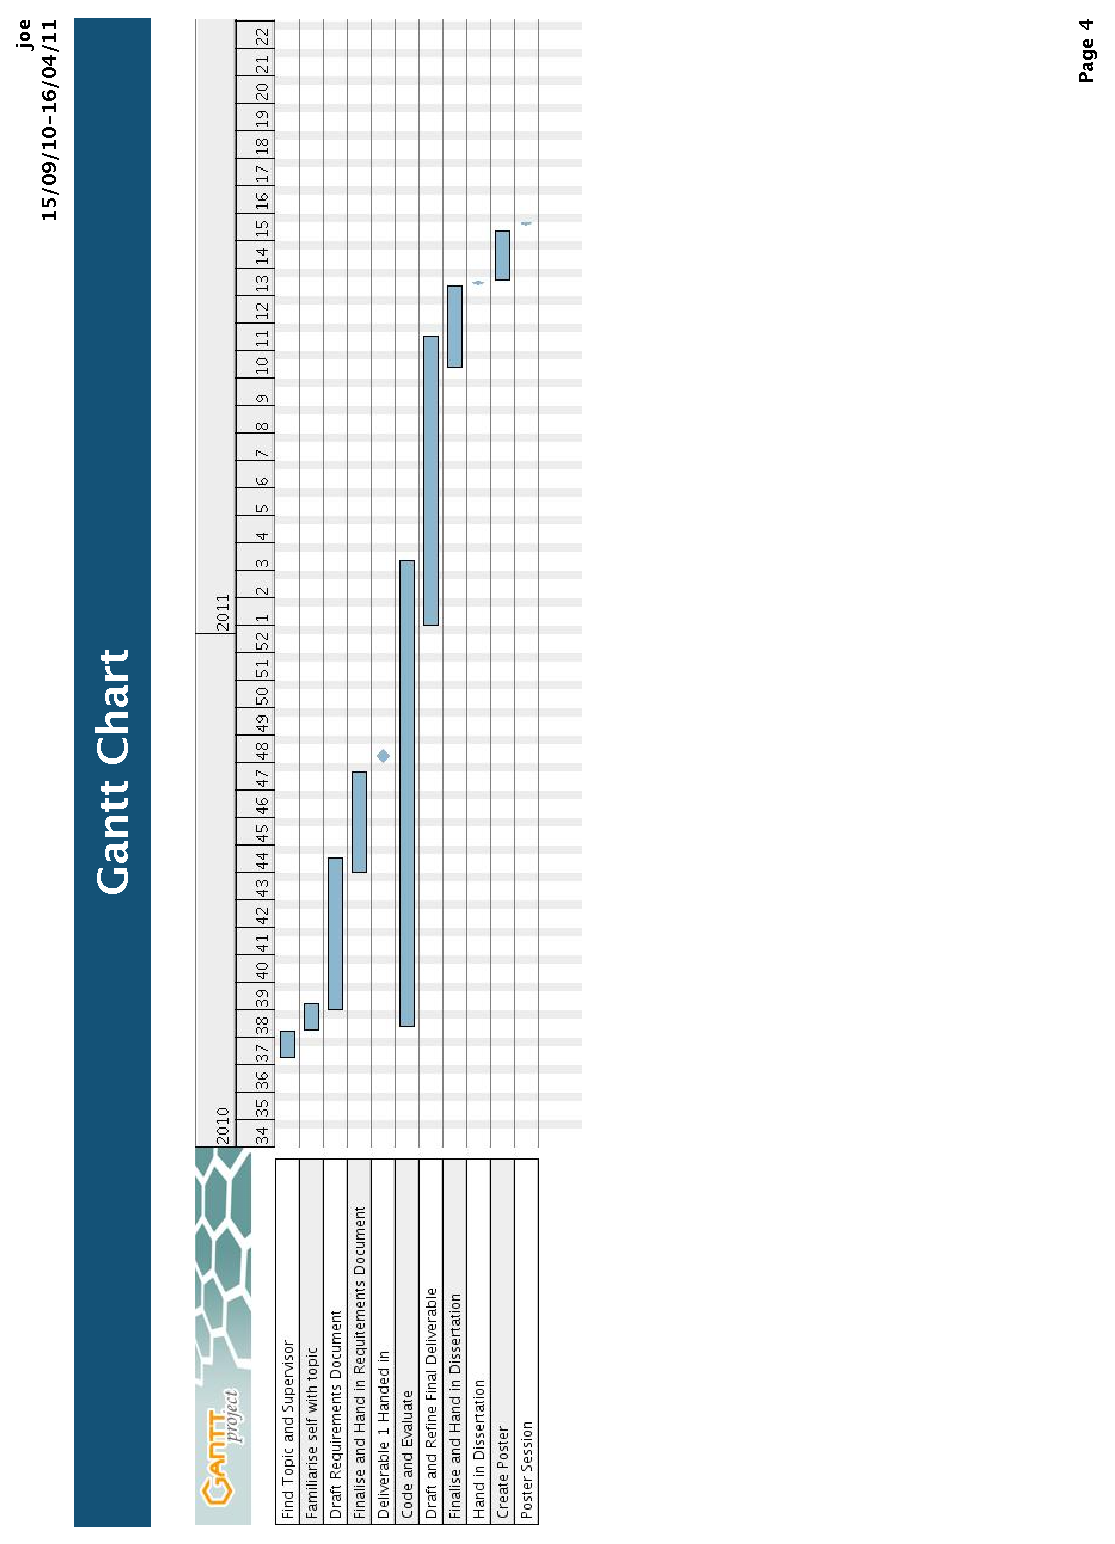
\includegraphics[trim=66 0 160 80,clip, height=16cm, width=9cm, angle=-90]{chart.eps}
      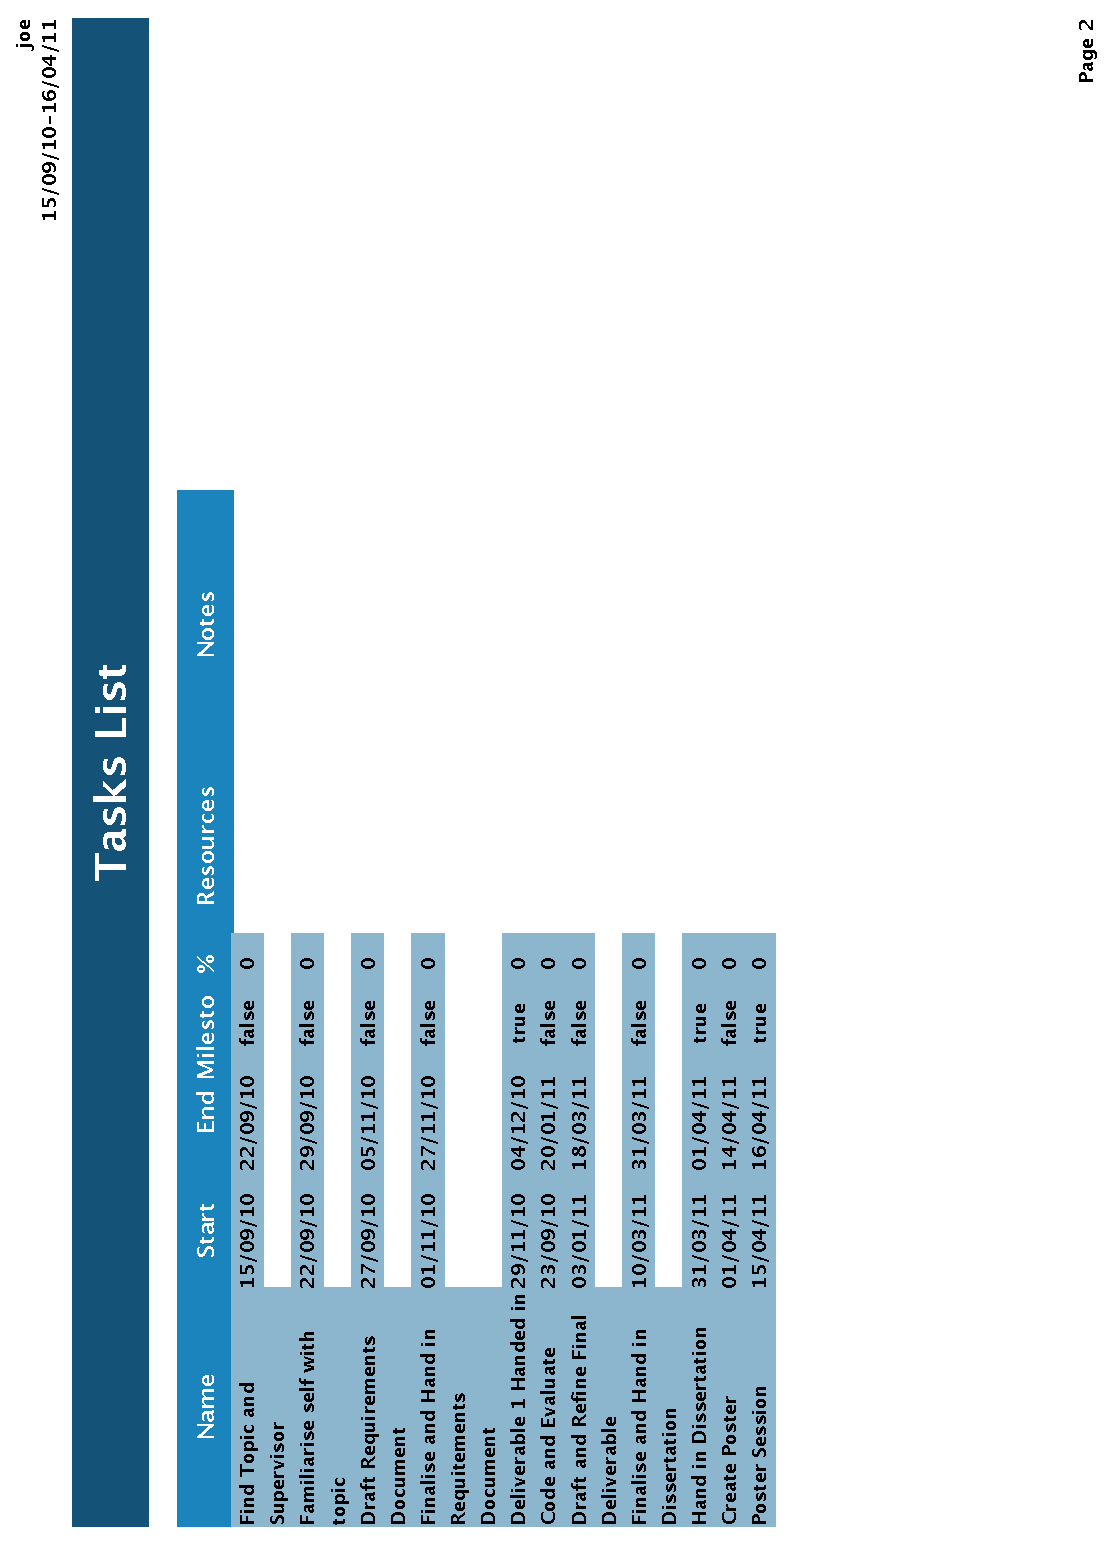
\includegraphics[trim=66 0 100 460,clip, width=10cm, angle=-90]{timetable.eps}
    \end{figure}

  \bibliographystyle{alpha}
  \bibliography{citation}
\end{document}
